\begin{chap}{First Projects}
%
\begin{sect}{Pseudosimilar Vertices}
%
\begin{para}
Vertices $u$ and $v$ in a graph $X$ are \textsl{similar} if there is an automorphism
of $X$ that maps $u$ to $v$. If $u$ and $v$ are similar, then the vertex-deleted
subgraphs $X\diff u$ and $X\diff v$ are isomorphic. If $X\diff u$ and $X\diff v$ 
are isomorphic but $u$ and $v$ are not similar, we say that they are
\textsl{pseudosimilar}. It is not obvious that pairs of pseudosimilar vertices
exist, but we will see that they do.
\end{para}
%
\begin{sagecode}
\begin{sageinput}
C9 = graphs.CycleGraph(9); C9
\end{sageinput}
\begin{sageoutput}
Cycle graph: Graph on 9 vertices
\end{sageoutput}
\end{sagecode}
%
\begin{para}
The vertex set of $C9$ is $\{0,\ldots,8\}$. We want to add three new vertices
to $C9$, adjacent to $1$, $4$ and $7$ in turn and delete the vertex $0$.
\end{para}
%
\begin{sagecode}
\begin{sageinput}
D = C9.copy()
D.add_edges([(1,9), (4,10), (7,11)])
D.delete_vertex(0)
\end{sageinput}
\end{sagecode}
%
\begin{para}
Here's $D$:
\end{para}
%
\begin{para}
% D.plot( layout='spring')
% No longer centered, lost 80% scaling
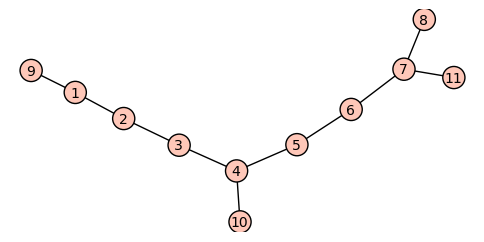
\includegraphics{graphplot.png}
\end{para}
%
\begin{para}
The automorphism group of $D$ has order 2:
\end{para}
%
\begin{sagecode}
\begin{sageinput}
D.automorphism_group().order()
\end{sageinput}
\begin{sageoutput}
2
\end{sageoutput}
\end{sagecode}
%
\begin{para}
and we can determine its orbits:
\end{para}
%
\begin{sagecode}
\begin{sageinput}
D.automorphism_group(return_group=False, orbits=True)
\end{sageinput}
\begin{sageoutput}
[[1], [2], [3], [4], [5], [6], [7], [8, 11], [9], [10]]
\end{sageoutput}
\end{sagecode}
%
\begin{para}
As an alternative to the last command we could try the following, but its
output is misleading!
\end{para}
%
\begin{sagecode}
\begin{sageinput}
D.automorphism_group().orbits()
\end{sageinput}
\begin{sageoutput}
[[1], [2], [3], [4], [5], [6], [7, 10], [8], [9], [11]]
\end{sageoutput}
\end{sagecode}
%
\begin{para}
This is because automorphism groups of graphs do not always exactly match the integer symbols for the permutation group to the names of the vertices.  Here is the translation between vertex names to permutation group symbols, as a Python dictionary.
\end{para}
%
\begin{sagecode}
\begin{sageinput}
D.automorphism_group(return_group=False, translation=True)
\end{sageinput}
\begin{sageoutput}
{1: 11, 2: 1, 3: 2, 4: 3, 5: 4, 6: 5, 7: 6, 8: 7, 9: 8, 10: 9, 11: 10}
\end{sageoutput}
\end{sagecode}
%
\begin{para}
I claim $D$ has a pair of pseudosimilar vertices. In this case we could find them
by inspecting our drawing of $D$, but we work through a general approach.
The idea is to find a canonical label for each of the 11 vertex-deleted subgraphs
of $D$. The sage command
\end{para}
%
\begin{sagecode}
\begin{sageinput}
E = D.canonical_label()
E.edges(labels=False)
\end{sageinput}
\begin{sageoutput}
[(0, 10), (1, 10), (2, 8), (3, 9), (4, 6), 
(4, 10), (5, 7), (5, 8), (6, 9), (7, 9)]
\end{sageoutput}
\end{sagecode}
%
\begin{para}
returns a canonized form of $D$. So graphs $G$ and $H$ are isomorphic if and only if
their canonized forms are equal. For example
\end{para}
%
\begin{sagecode}
\begin{sageinput}
P = graphs.PetersenGraph()
Q = graphs.CompleteGraph(5).line_graph().complement()
Pc = P.canonical_label(); Qc = Q.canonical_label()
P == Q, Pc == Qc
\end{sageinput}
\begin{sageoutput}
(False, True)
\end{sageoutput}
\end{sagecode}
%
\begin{para}
The only problem left is that the return value of \verb|canonical_label()|
is not hashable. We can circumvent this as follows.
\end{para}
%
\begin{para}
The following procedure constructs a hashable canonical label for 
$G\diff i$, given $G$ and $i$.
\end{para}
%
\begin{sagecode}
\begin{sageinput}
def vdi(G, i):
    H = G.copy()
    H.delete_vertex(i)
    return (H.canonical_label().graph6_string(), i)
\end{sageinput}
\end{sagecode}
%
\begin{para}
We can now construct our list of pairs of the form (string, vertex):
\end{para}
%
\begin{sagecode}
\begin{sageinput}
orbs = D.automorphism_group( return_group=False, orbits=True)
orb_reps = [it[0] for it in orbs]
labels = [vdi(D,i) for i in orb_reps]
labels
\end{sageinput}
\begin{sageoutput}
[('I??G?DaDO', 1), ('I_???CpB_', 2), ('I??X??BoO', 3), 
('I???GOPW_', 4), ('I??G_GBw?', 5), ('I??X??BoO', 6), 
('I???Gg_Ag', 7), ('I??OQaGH_', 8), ('I???oH`b?', 9), 
('I?COOIAWO', 10)]
\end{sageoutput}
\end{sagecode}
%
\begin{para}
and on inspecting the output, we see that $D\diff 3\cong D\diff 6$.
\end{para}
%
\begin{para}
As an exercise, construct a graph on 8 vertices with a pair of pseudosimilar
vertices.
\end{para}
%
\begin{para}
Now we describe how to get a list of the sets of vertices such that all
vertices in the same set have the same vertex-deleted subgraphs.
First we need to convert our list of pairs to a dictionary keyed on the 
first term of the pair; the value of a key will be all second terms 
with the same first term. (The keys for a dictionary must be hashable, so this
is why we needed the graph6 strings.)
\end{para}
%
\begin{sagecode}
\begin{sageinput}
def ls_dict( tuples):
    dc = {} 
    for pair in tuples:
        if dc.has_key( pair[0]):
            dc[ pair[0]].append(pair[1])
        else:
            dc[ pair[0]] = [pair[1]]
    return dc
\end{sageinput}
\end{sagecode}
%
\begin{para}
Now if \verb|dc| is a dictionary whose values are lists, we compute a list consisting
of those values whose length is at least $k$:
\end{para}
%
\begin{sagecode}
\begin{sageinput}
def get_families( dc, k):
    families = []
    for str, vxs in dc.iteritems():
        if len(vxs) >= k:
            families.append( vxs)
    return families
\end{sageinput}
\end{sagecode}
%
\begin{para}
We apply this to our list \texttt{labels}:
\end{para}
%
\begin{sagecode}
\begin{sageinput}
get_families( ls_dict( labels), 2)
\end{sageinput}
\begin{sageoutput}
[[3, 6]]
\end{sageoutput}
\end{sagecode}
%
\begin{para}
We see again that 3 and 6 form a pseudosimilar pair of vertices.
\end{para}
%
\begin{para}
For further reading on pseudosimilar vertices, you will have to dig out papers
on the topic.  I suspect that few of these are on the web, since they
predate \LaTeX{}.  Fortunately we still have libraries.  Note that pseudosimilar
sets of size greater than two are possible.
\end{para}
%
\end{sect}
%
\begin{sect}{Circle Graphs}
%
\begin{para}
To construct a \textsl{circle graph} we first choose $n$ pairs of points on a 
circle in the real plane and then join each pair of points by a straight line,
a \textsl{chord}. These chords are the vertices of the circle graph and they
are adjacent if and only if they cross.
\end{para}
%
\begin{para}
In fact we can view our $2n$ points as the vertices on the cycle of length
$2n$, and represent the chords by a perfect matching in the complete graph
on the vertices of the cycle. We call this structure a \textsl{chord diagram}.
This can be viewed as a cubic graph, with a parallel edge wherever the matching
edge is also an edge in the cycle.
Since a matching edge which is parallel to a cycle edge does not cross
another matching edge, it forms an isolated vertex in the circle
graph. For most purposes we can therefore assume that the matching has
no edge in the cycle---it's a subgraph of $\comp{C_{2n}}$.
\end{para}
%
\begin{para}
Chord diagrams arise in knot theory. Suppose we have a knot drawn in the
plane; assume that there are $n$ crossings labelled 1 through $n$. The knot is 
an embedding of a circle and, on walking around this circle we see a sequence
of $2n$ integers. The terms of the sequence are elements of $\{1,\ldots,n\}$,
and each element occurs twice. Such a sequence is known as a 
\textsl{double occurrence word}. We could even encode the actual knot by
assigning $i^+$ to the overpass and $i^-$ to the underpass, but we digress.
Each double occurrence word determines a chord diagram with $n$ chords---
simply write the word on the vertices of $C_{2n}$ in the natural way, and then
join vertices with the same label by an edge.
\end{para}
%
\begin{para}
For the moment at least, we specify a circle graph on $n$ vertices by a 
perfect matching in $K_{2n}$, and thus by a set of $n$ edges.
We need to decide if two edges of the matching cross:
\end{para}
%
\begin{sagecode}
\begin{sageinput}
def cross(e1,e2):
    if e1[1]<e1[0]: e1[0],e1[1] = e1[1],e1[0]
    if e2[1]<e2[0]: e2[0],e2[1] = e2[1],e2[0]
    return (e1[0]<e2[0] and e2[0]<e1[1]<e2[1]) or (e2[0]<e1[0]<e2[1] and e2[1]<e1[1])
\end{sageinput}
\end{sagecode}
%
\begin{para}
With this in hand we can easily construct the circle graph corresponding
to a given matching:
\end{para}
%
\begin{sagecode}
\begin{sageinput}
def circle_grf(pm):
    return Graph([range( len( pm)), lambda i,j: cross(pm[i],pm[j])])
\end{sageinput}
\end{sagecode}
%
\begin{sagecode}
\begin{sageinput}
def chord_dgrm(pm):
    dgrm = graphs.CycleGraph( 2*len(pm))
    dgrm.add_edges( pm)
    return dgrm
\end{sageinput}
\end{sagecode}
%
\begin{sagecode}
\begin{sageinput}
pm = [(0, 8), (1, 4), (2, 9), (3, 6), (5, 7)]
CD = chord_dgrm( pm)
show(CD)  # not tested
\end{sageinput}
\begin{sageoutput}
\end{sageoutput}
\end{sagecode}
%
\begin{para}
We can get the perfect matchings in the complement of $C_{10}$ as follows.
(It's not pretty, but it works.)
\end{para}
%
\begin{sagecode}
\begin{sageinput}
C = graphs.CycleGraph(10)
CC = C.complement().line_graph().complement()
cliques = CC.cliques_maximum()
len(cliques)
\end{sageinput}
\begin{sageoutput}
293
\end{sageoutput}
\end{sagecode}
%
\begin{para}
So there are 293 perfect matchings in the complement of $C_{10}$. It is easy
to create the corresponding circle graphs and then find the number of different possibilities by examining canonical labelings.
\end{para}
%
\begin{sagecode}
\begin{sageinput}
grfs = [circle_grf( pm).canonical_label().graph6_string() for pm in cliques]
uniq = Set(grfs)
uniq
\end{sageinput}
\begin{sageoutput}
{'DBk', 'D]{', 'D`K', 'DK[', 'DBg', 'DB{', 
'D@s', 'D^{', 'D@{', 'D?{', 'Dbk', 'DF{', 
'DIk', 'D@O', 'DJ{', 'DLo', 'DK{', 'D~{', 
'D_K', 'DNw', 'DL{', 'DJk', 'DFw', 'DN{'}
\end{sageoutput}
\end{sagecode}
%
\begin{para}
With just 24 different circle graphs resulting from the 293 matchings, we see this is not a particularly efficient way to generate circle graphs.
\end{para}
%
\begin{para}
We can make use of procedures to convert between perfect matchings and double
occurrence words.
\end{para}
%
\end{sect}
%
\begin{sect}{Line Graphs and Covers}
%
\begin{para}
Let $D$ be the incidence matrix of an orientation of the graph $X$. Then
\[
    DD^T = \De -A,\quad D^TD = 2I +S
\]
where $\De$ is the diagonal matrix of valencies of $X$ and $S$ is a symmetric
matrix with zero diaogonal and off-diagonal entries from $\{0,1,-1\}$.
In other words, $S$ is a \textsl{signed adjacency matrix}. The entries of
$S$ are indexed by $E(X)$, and the $ab$-entry is non-zero if and only if
the edges $a$ and $b$ are adjacent in the line graph $L(X)$ of $X$,
so we have a signed adjacency matrix for $L(X)$.
\end{para}
%
\begin{para}
A signed ajacency matrix $T$ of a graph $Y$ determines a \textsl{two-fold cover} $Z$
of $Y$, as follows. The vertex set of the cover is
\[
    V(Y) \times \{0,1\}
\]
and $(u,i)$ and $(v,j)$ are adjacent if and only if $u\sim v$ and either
\[
    i=j,\quad T_{u,v}=1
\]
or
\[
    i\ne j,\quad T_{u,v}=-1.
\]
It is easy to check that the map that sends $(u,i)$ to $(u,1-i)$ is an automorphism
of $Z$. In matrix terms, we get the adjacency matrix of $Z$ by applying
the following substitutions to the entries of $A(Y)$:
\[
    0\to\pmat{0&0\\0&0},\qquad 1\to\pmat{1&0\\0&1}
        \qquad -1\to\pmat{0&1\\1&0}.
\]
\end{para}
%
\begin{para}
The pairs 
\[
    \{(u,0),(u,1)\}
\]
are called the fibres of the cover, you might verify that these form an equitable
partition of the cover, and that the quotient over the fibres is $Y$. Thus
we see that the characteristic polynomial of the cover is divisible
by the characteristic polynomial of the graph.
\end{para}
%
\begin{para}
%
\begin{lemma}
\begin{statement}
\[
        \phi(Z,t) =\phi(T,t)\phi(Y,t).
\]
\end{statement}    
\begin{proof}
(Outline.) Let $H$ be the matrix
\[
    \frac{1}{\sqrt{2}} \pmat{1&1\\1&-1}
\]
and let $K$ be the block-diagonal matrix formed using $|V(Y)|$ copies of $H$.
If $M$ is a complex matrix, let $|M$ denote the matrix we get by replacing each entry
of $M$ by its absolute value.
Then $K$ is orthogonal and symmetric and $KA(Z)K$ is permutation equivalent to 
\[
    \pmat{S&0\\0&|S|}.
\]
\end{proof}
\end{lemma}
\end{para}
%
\begin{para}
Here $|S|=A(Y)$. We offer another view of this result.
If $A$ and $B$ are symmetric $01$-matrices such that $A\circ B=0$,
then $A-B$ is a signed adjacency matrix and
\[
    \pmat{A&B\\B&A}
\]
is the adjacency matrix of the corresponding cover.
We can now use the following:
\[
    \frac12\pmat{I&I\\I&-I}\pmat{A&B\\B&A}\pmat{I&I\\I&-I}
        =\pmat{A+B&0\\0&A-B}.
\]
\end{para}
%
\begin{para}
This leads us to an easy construction of the adjacency matrix of the cover.
\end{para}
%
\begin{sagecode}
\begin{sageinput}
def lgcvr( X):
    D = X.incidence_matrix()
    IDM = identity_matrix( X.num_edges())
    M = D.transpose()*D -2*IDM
    MM = M.elementwise_product(M)
    A = (1/2)*(M+MM)
    B = (1/2)*(M-MM)
    return block_matrix(2, 2, [A,B,B,A])
\end{sageinput}
\end{sagecode}
%
\begin{para}
Now we turn to our line graphs. The cover can be constructed as follows.
Choose one arc $(u,v)$ for each edge $\{u,v\}$ of $X$. (This defines an orientation
of the graph.) Our matrix $S$ is a signing of $A(L(X))$---its rows and columns
are indexed by our chosen arcs, and the entry corresponding to a pair
of distinct overlapping arcs is 1 if they have the same head or tail,
and $-1$ otherwise. Rather than represent the vertices of the cover by
pairs $((u,v),i)$, we proceed thus: if $(u,v)$ is one of our chosen
arcs then we use $(u,v)$ to denote $((u,v),0)$ and $(v,u)$ for $((u,v),1)$.
The following procedure implements this.
\end{para}
%
\begin{sagecode}
\begin{sageinput}
def dbl_lng( X):
    V = X.vertices()
    E = X.edges( labels=False)
    arcs = [(i,j) for i in V for j in V\
        if ((i,j) in E or (j,i) in E)]
    return  Graph( [arcs, lambda a,b: a != b and (a[0]==b[0] or a[1]==b[1])])
\end{sageinput}
\end{sagecode}
%
\begin{para}
We test that our two constructions agree on the Petersen graph, and see
that cover is isomorphic to the line graph of the direct product of
the Petersen graph with $K_2$. (This product is itself a cover of the Petersen
graph.)
\end{para}
%
\begin{sagecode}
\begin{sageinput}
P = graphs.PetersenGraph()
Q1 = Graph( lgcvr( P))
Q2 = dbl_lng( P)
Q1.is_isomorphic( Q2)
\end{sageinput}
\begin{sageoutput}
True
\end{sageoutput}
\end{sagecode}
%
\begin{sagecode}
\begin{sageinput}
K2 = graphs.CompleteGraph(2)
LP2 = (P.tensor_product(K2)).line_graph()
LP2.is_isomorphic( Q1)
\end{sageinput}
\begin{sageoutput}
True
\end{sageoutput}
\end{sagecode}
%
\end{sect}
%
\end{chap}